%Linea Para poder completar automaticamente las citas con el Sublime
%No hace el documento, se puede borrar esta linea si no se usa el Sublime
%------------------------------------------------------------------------------
 \newcommand{\NoBiblioEQ}[1]{
 \ifthenelse{\equal{#1}{verdadero}}{}{\bibliography{Referencias/base_bibliografica}}
 \NoBiblioEQ{verdadero}}
 %----------------------------------------------------------------------------- 

%Formato (Nombre de capitulo largo o corto), nombre del capitulo y estilo de la
%Portada del Capitulo
%------------------------------------------------------------------------------

 %Formato en si, titulo en un solo renglon
 \FormatoCapituloDosLineas
 
 %Nombre y etiquete para referir
 \chapter{Propiedades de transporte de los sensores}
 \label{chap:Electroquimica}

 %Para que no salga el numero de pagina en la portada del capitulo
 \thispagestyle{empty}
	
 %Resumen del Capitulo en Italica
 \noindent\textit{Aca va todo el desarrollo de la fisicoquimica de los mesospororos, fenomenos de  transporte, adsorcion, Langmuir, propiedades de mediacion redox, catalisis, etc, etc.}

 %Indice de capitulo alineada al borde inferior de la pagina, nueva pagina
 \vfill
 \minitoc
 \newpage
 %-------------------------------------------------------------------------------

\section{Introducción}

	Una vez estudiados los distintos tratamientos de síntesis y realizada la fabricación de los sensores se dedicará, en este capitulo, a estudiar las propiedades de los mismos para detectar y cuantificar una serie de sondas electroquímicas elegidas, precisamente, para poder evaluar distintos aspectos de transporte a través de los sistemas nanoporosos. 
	Los sensores están compuestos básicamente de una película delgada de oro y una película delgada nanoporosa de SiO$_2$. 

	La superficie de las paredes dejan expuestos, hacia el interior de los poros, grupos silanoles los cuales pueden estar o no protonados.\cite{Brinker1990,Soler-Illia2011} 
			\begin{equation}
				\begin{aligned}
				\includegraphics[scale=0.75]{Esquemas/equilibriosilica.pdf}
				\label{eq:equilibriosilica}
				\end{aligned}
				\end{equation}

	La reacción \ref{eq:equilibriosilica} ejemplifica el equilibrio ácido-base que se establece en la superficie de la sílice. El pKa del $\text{SiO}_2$ es menor a 4 y la mayoría de los autores coinciden en que el punto isoeléctrico (PI) varía de $1$ a $4$ dependiendo de  las distintas forma alotrópicas del óxido de silicio, en particular para el SiO$_2$ sintetizado vía sol-gel el $\text{PI}\approx 2$ \cite{Kosmulski2002,Kosmulski2014,Schwarz1984,Si-HanWu2013}.
	Wu y colaboradores\cite{Si-HanWu2013} analizaron, por un lado, el estado de carga superficial de nanoparticulas de sílice mesoporosa y, por otro, la tasa de condensación. El gráfico de la figura \ref{fig:silica_ph} muestra como varían las razones  $\text{SiO}^{-}/\text{SiOH}$ y $\text{SiOH}_2^{+}/\text{SiOH}$ en función del pH; se puede apreciar que solo por encima de $\text{pH}\geq7$ se obtiene una superficie de carga negativa donde todos los silanoles reaccionaron, cediendo su $\text{H}^{+}$, para convertirse en iones silanoatos; mientras que para pH bajos ($\text{pH}\leq1$), la sílice se vuelve inestable antes de llegar a un estado de carga completamente positivo y, solo queda, parcialmente positiva. En el mismo trabajo\cite{Si-HanWu2013} también plantean que la tasa de condensación decrece por encima de $\text{pH}\geq7.5$ debido a entra en una zona de inestabilidad donde el óxido se disuelve, catalizado por el medio básico.
			\begin{figure}[th!]
			\centering
 	       	\includegraphics[width=0.70\textwidth]{Graficos/Silica-PH-Stability.pdf}
	       		\caption[Tasa de condensación y estado de carga superficial]{Tasa de condensación y estado de carga superficial para nanoparticulas de sílice en función de pH. Gráfico extraído de \textit{Synthesis of mesoporous silica nanoparticles} Chem. Soc. Rev., 42(9):3862, 2013.\cite{Si-HanWu2013}}
	         	\label{fig:silica_ph}
	     		\end{figure}
			
	%Del equilibrio se desprende que al incrementar el pH por encima de $2$ la película presentará una carga neta negativa, y, consecuentemente al disminuir el pH por debajo de $2$ la película será neutra o levemente positiva. 
	De hecho, Iler, en su libro \textit{<<The Chemistry of Silica>>}, explica que la tasa de disolución de la sílice en medio acuoso depende de muchos factores y, que además, salvando el tipo de sílice, el proceso de disolución requiere de un catalizador. Presenta un gráfico de la tasa de disolución en función del pH (figura \ref{fig:disolucion_ph}) y postula que la tasa de disolución depende de la forma alotropica de la sílice, mientras que para formas mas porosas como el SiO$_2$ amorfo la cinética de disolución es mas rápida, para otras como el cuarzo se hace mucho mas lenta; por último aclara que se trata de un proceso de despolimerización vía hidrólisis, y la solubilidad es la concentración de Si(OH)$_4$ cuando alcanza un estado estacionario en el equilibrio despolimerazación-polimerización.\cite{iler1979}. 

			\begin{figure}[th!]
			\centering
 	       	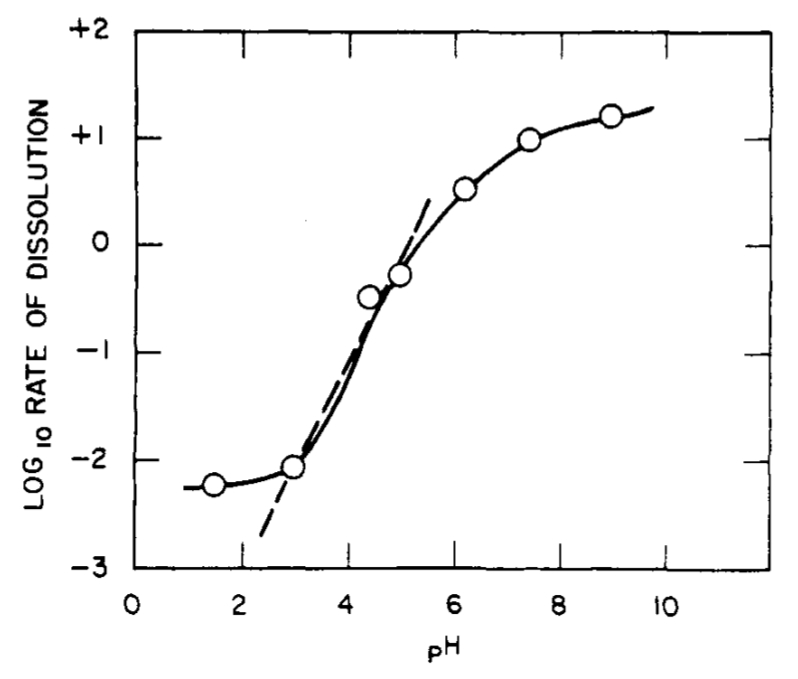
\includegraphics[width=0.70\textwidth]{Graficos/disolucion_ph.pdf}
	       		\caption[Tasa de disolución sílice en función del pH]{Tasa de disolución de la sílice en función de pH. Gráfico extraído de \textit{The chemistry of silica} Wiley 1ª edición, 1979.\cite{iler1979}}
	         	\label{fig:disolucion_ph}
	     		\end{figure}
	
	También propone un mecanismo en medio ácido catalizado por iones F$^-$, mientras que en medio básico el mecanismo es catalizado por iones OH$^-$, según el siguiente mecanismo:
			\begin{equation}
				\begin{aligned}
				\includegraphics[scale=0.60]{Esquemas/disolucionsilica.pdf}
				\label{eq:disolucionsilica}
				\end{aligned}
				\end{equation} 
	
	El mecanismo de \ref{eq:disolucionsilica} no está completamente consensuado en la literatura especializada, sin embargo todos los autores coinciden en que el óxido se vuelve inestable en cualquiera de sus forma alotrópicas a partir de un $\text{pH}\geq7$ y que, a partir de $\text{pH}\geq10$ el proceso de disolución se acelera considerablemente varios ordenes de magnitud.\cite{Kosmulski2002,Kosmulski2014,Schwarz1984,Si-HanWu2013,iler1979}

	%Dependencia de la constante de K con el PH.... poner aqui el grafico, ecuacion y grafico de Wu2013 donde propone estado de carga y donde se muestra que recien a PH=5 se llega a un estado de carga copmpeltamente negativo.
	
				
	%ca tengo que poner como es la reaccion del punto isoeléctrico del Sio2 o del punto de carga zero... o del pka??? Y tambien tengo que poner los antecendente de calvo, calvo y el otro del 2005. Y tambien entonces que la diferencia es el Au miniaturizacion, etc, etc mayores velocidades... etc. 
	%No olvidarse de los ferrocenos a distintas velociades de barrido

\section{Transporte de sondas: exclusión, permeación y preconcentración}

	Durante las próximas secciones se analizan e interpretan los resultados obtenidos al colocar soluciones con sondas electroquímicas, de diferente naturaleza, sobre los sensores. Al ser, la fabricación de los sensores, una parte estructural de este trabajo, cabe aclarar sobre que sistemas que se realizaron los resultados de los experimentos que se mostrarán de este capitulo; se utilizó, indistintamente, películas de Au sobre sustratos varios (silicio, vidrio, flexible), con diseño ya transferido o sin transferir. Salvo que se aclare lo contrario, se trabajó siempre sistemas con películas delgadas mesoporosas estructuradaras con Pluronic F127 y sintetizada con el método de alto vacío (consultar sección \ref{sec:trat-vacio}, pág. \pageref{sec:trat-vacio}); todas las medidas fueron normalizadas por el área geométrica, de forma de facilitar la comparación de resultados cuando se trata de sensores con distinto diseño; todas las medidas fueron llevadas a cabo a $\text{pH}\approx5,5$ en solución de KCl \SI{100}{\milli\Molar}, elegido con el propósito de mantener una fuerte carga neta negativa dentro de la películas, y a su vez, no estar comprometer la disolución de la sílice.

	\subsection{Caso 1: sonda de carga negativa}

	El voltagrama de la figura \ref{fig:exclusion_vs_Au} muestra la respuesta de los sensores cuando se colocan en una solución con una sonda negativa. Como sonda de carga negativa se utilizó ferro/ferriciunuro de potasio (\ferroferri, \SI{1}{\milli\Molar}) en proporciones equimolares. El voltagrama rojo corresponde a la respuesta en un electrodo de Au desnudo, mientras que la verde a un electrodo recubierto de \pdm.
	
			\begin{figure}[ht]
				\centering
		 	    \includegraphics[width=0.70\textwidth]{Graficos/ExclusionFcCN.pdf}
		        \caption[Exclusión electrostática]{Respuesta compartiva de un electrodo de Au recubierto con \pdmF\space y sin recubrir frente a una sonda \ferroferri \SI{1}{\milli\Molar} en \SI{0.1}{\Molar} de KCl contra ESC.}
		        \label{fig:exclusion_vs_Au}
		      	\end{figure}
	
	 Al ser la sonda de carga negativa, no es capaz de ingresar a la película (la cual está cargada negativamente), y, por lo tanto tampoco puede difundir hacia el electrodo, eso se refleja en el voltagrama donde no se observa ni reducción ni oxidación de la sonda. La repulsión se debe a un efecto de exclusión electrostática. Este fenómeno de exclusión ya fue reportado por varios autores\cite{alberti2015,schmuhl2005,Andrieu-Brunsen2015,brunsen2011}. Al pH de trabajo, $\text{pH}=5,5$, los silinanoles están como silanolatos, como ya se explicó anteriormente, estableciendo una carga negativa en todo el espesor de la película.

	 Desde el punto del estudio de fenómenos de  transporte esta sonda no es especialmente útil, porque, como ya se demostró, no puede ingresar en la \pdm. Sin embargo, nos ofrece información importante sobre la integridad estructural de las películas delgadas, dicho de otro modo, al no obtener señal electroquímica significa que, la sonda no percola a través de la \pdm, que la \pdm\space se encuentra sin fisuras, agujeros o rajaduras y que recubre por completo el área del electrodo.

	 Por ende fue muy importante para corroborar (si no hay señal la película esta intacta, si hay señal esta el Au expuesto) el estado de las \pdm\space al finalizar experimentos donde se dudaba del estado de la película, de esta forma se utilizó esta sonda a modo de <<experimento control>>, realizando una voltametría cíclica para comprobar que las películas no tuviera sitios de percolación.

	\subsection{Caso 2: sonda de carga neutra}

		Al ser el ferroceno metanol una molécula que, en su estado reducido, no presenta carga, es de esperar que no se vea afectada por la carga que presentan las paredes de los poros. En la figura \ref{fig:permeacion} se comparan los voltagramas resultantes de colocar una solución de ferroceno matanol sobre un electrodo de Au desnudo (voltagrama rojo) y uno recubierto con la \pdm.  Si bien el gráfico  requiere mas análisis, está claro que el ferroceno permea a través de la película nanoporosa, para dar una señal electroquímica. En las próximas secciones se discutirá la forma, intensidad y otras variables de los voltagramas, y se analizarán experimentos complementarios, por ahora basta con haber demostrado que una sonda neutra atraviesa la \pdm\space para dar una señal electroquímica, unas cuatro veces menor que la respectiva señal en un electrodo de Au desnudo.	

		\begin{figure}[ht]
				\centering
		 	    \includegraphics[width=0.70\textwidth]{Graficos/FeOH-permeacion-1mM.pdf}
		        \caption[Permeación ferroceno metanol]{Respuesta compartiva de un electrodo de Au recubierto con \pdmF\space y sin recubrir frente a una sonda \fc \SI{1}{\milli\Molar} en \SI{0.1}{\Molar} de KCl contra ESC.}
		        \label{fig:permeacion}
		      	\end{figure}
		%Ferroceno y todos los datos de permeacion. Calcinado vs Bajas Tcd 

	\subsection{Caso 3: sonda de carga positiva}

	Para este caso se utilizó como sonda cloruro de hexaminorutenio (III), sonda bien conocida por su reversibilidad entre los estados reducido y oxidado. Los primeros experimentos con está sonda dan como resultados los voltagramas de la figuras \ref{fig:Ru10mM}. Allí se muestran los resultados de realizar una serie continua de sucesivas voltametrías cíclicas y seguir su evolución en el tiempo, desde el verde claro al verde oscuro. El cambio en la señal en función del tiempo se debe al ingreso el \aminorutenio\space a través de la matriz porosa, aumentando la intensidad de la señal conforme aumenta la concentración de la sonda dentro de los poros. A su vez, también se observa un desplazamiento hacia un potencial mas reductor del pico anódico, esto indica que parte \aminorutenio\space se está adsorbiendo dentro de los poros, consecuencia de una interacción electrostática sonda-pared, generando una señal <<mixta>> con dos contribuciones, la del \aminorutenio\space libre en solución o libre dentro de los poros y la del adsorbido en las paredes de la película mesoporosa, esto se ve claramente en los voltagramas de la figura \ref{fig:Ru10mM-resumen}.

	Para poder separar estas contribuciones se realizó el siguiente experimento. Una vez alcanza la intensidad de pico máxima se retira de la celda la solución con la sonda, y se reemplaza por solución que contiene únicamente electrolito soporte, de esta forma, de existir señal, solo tendría sentido si la misma se debe al \aminorutenio\space retenido en la película mesoporosa. El gráfico de la figura \ref{asd} muestra los resultados de dicho experimento, el mismo contiene tres voltagramas; el color rojo corresponde a la respuesta de \aminorutenio\space en un electrodo de Au desnudo; la curva de color verde a la señal de una película <<cargada>> de \aminorutenio\space con solución de \aminorutenio; y la curva azul es el resultado de intercambiar la solución son la sonda por solución con electrolito soportes unicamente. Esta última curva tiene la forma características que presentan las sondas adsorbidas o matrices con sitios redox <<anclados>>, como los que presentan los polímeros conductores \cite{Ybarra2005} o los polímeros funcionalizados con compuestos electroactivos \cite{Rohlfing2005,Vila2015}, donde la separación de potencial entre los picos catodicos y anodicos es menor que \SI{60}{\milli\volt}, $\Delta E < \SI{60}{\milli\volt}$ 

			\begin{figure}[ht!]
				\begin{subfigure}[t]{0.495\textwidth}
				\includegraphics[width=1\textwidth]{Graficos/Ru10mM-ads-libre-flecha.pdf}
		        \caption{Ingreso de \aminorutenio\space \SI{10}{\milli\Molar} en una \pdmF.}
		        \label{fig:Ru10mM_ingreso}
		      	\end{subfigure}
		      	\begin{subfigure}[t]{0.495\textwidth}
				\includegraphics[width=1\textwidth]{Graficos/Ru10mM-Resumen.pdf}
		        \caption{Voltagramas donde se compara la señal en Au (\usebox{\rojo}), en una \pdmF\space(\usebox{\oliva}) y en una \pdmF\space luego de retirar la solución de \aminorutenio (\usebox{\azul}).}
		        \label{fig:Ru10mM-resumen}
		      	\end{subfigure}
		      	\caption[Adsorción de sonda positiva en \pdm]{Solución de \aminorutenio\space \SI{10}{\milli\Molar} en KCl \SI{100}{\milli\Molar} a $\text{pH}=5,5$. En a) se ve como aumenta la señal mientras la sonda ingresa en la estructura porosa, en b) se muestra el adsorbido versus libre}
		      	\label{fig:Ru10mM}
		      	\end{figure}


	Sin duda,  este es el caso mas interesan de los tres expuestos y el mas interesante para estudiar propiedades físicas y químicas del sistema, estudiar fenómenos de transporte o variables del sistema. Es por ello que las proximas secciones se basarán en este caso,
 	      	      		      	

	\section{Caso de estudio: cloruro de hexaminorutenio}
		


	se basaron en trabajos que utilizan, o esta misma sonda\cite{} o sondas de rutenio bipiridina. Losresultados fue el gráfico  que se encuentra en la la fig \ref{fig:primera_adsorcion} dondes.... se muestra la evolacu¡on sucesivas CVs......... ingresa.... maximos..... disolcuion... tal como indican el hombro.

			
	En vista de estos resultados, lo primero que se hizo fue establecer donde es fiable trabajar antes de que se disuelva completamente la peliculas. Si bien estamos en a un PH donde la disolucion deberia ser minima o nula, las mismas parecen disolverse con bastante facilidad. De estos resultados surgio la incognita de si la disolucion se debe al pH a la sonda o a al potencial aplicado. La respuesta a esta pregunta se manifestó ..... grafico .... comparando... efecto combinado adsorcion y ingreso de iones.... No pasa con Ferroceno, HQ, permeacion.... clara exclusion del Ferro/Ferri. tambien ocurre en el calcinado.

			\begin{figure}[ht]
				\centering
		 	    \includegraphics[width=0.70\textwidth]{Graficos/Sondas-Tiempo-Disolucion.pdf}
		        \caption[AAAAAAaa]{Comparacion sondas.........¿¿¿debo poner la linea del Au en 1???}
		      	\end{figure}

	Conforme lo expuesto anterirmete, se trabajo en establecer las condiciones de contorno para las cuales sean validos los resultados obtenidos. Para ellos se establecion una ventana de trabajo donde es segura maxima adsorcion e integridad de la peliculas.
			
			\begin{figure}[th]
	 	   	    \begin{subfigure}[t]{0.325\textwidth}
		        	\includegraphics[width=0.95\textwidth]{Graficos/Ru10mM-ventana-preconcentracion.pdf}
		       		\caption{Ru10mM.}
		         	\label{fig:Ventana_Ru10mM}
		     		\end{subfigure}
	     		\begin{subfigure}[t]{0.325\textwidth}
		        	\includegraphics[width=0.95\textwidth]{Graficos/Ru1mM-secuencia-continua-hasta-disolucion-ventana-trabajo.pdf}
		       		\caption{Ru1mM.}
		         	\label{fig:Ventana_Ru1mM}
		     		\end{subfigure}
	     		\begin{subfigure}[t]{0.325\textwidth}
		        	\includegraphics[width=0.95\textwidth]{Graficos/Ru0315mM-secuencia-continua-ventana-trabajo.pdf}
		       		\caption{Ru 0.315mM}
		         	\label{fig:Ru_0315mM}
		     		\end{subfigure}
	 	   	   	\caption[asdasdasd]{asdasdasd}
	     		\label{fig:ventana-trabajo}
	     	   	\end{figure}

	Para corroborar que realmente se encuetre adosrbido se llevo a cabo un experimente en el cual luego de alcanzar el maximo de adsorcion se retira la solucion con la sonda y se reemplaza con solucion que contiene unicamente electrolito soporte, el resultado es la tipica curva para una especie adsorbida. donde se ve que el AE < 60. El grafico nos resume este experimento donde se comparan al amismo tiempo...... Au.... Au con meso y Adosorbido.... en el que se ve que contribuyen a la señal EQ dos aporte el adsrovido y el ru libre.

			\begin{figure}[ht]
				\centering
		 	    \includegraphics[width=0.70\textwidth]{Graficos/Ru10mM-Resumen.pdf}
		        \caption[asd]{Comparacion de Ru 10mM para .........}
		        \label{fig:asd}
		      	\end{figure}     	   	

		    	\begin{figure}[th]
		   	     \begin{subfigure}[t]{0.325\textwidth}
		        	\includegraphics[width=0.95\textwidth]{Graficos/Ru10mM.pdf}
		        	\vspace*{-0.40cm}\caption{Ru 10mM.}
		         	\label{fig:Ventana_Ru1mM}
		     		\end{subfigure}
		   	    \begin{subfigure}[t]{0.325\textwidth}
		        	\includegraphics[width=0.95\textwidth]{Graficos/Ru63mM.pdf}
		       		\vspace*{-0.40cm}\caption{Ru 6.3mM.}
		         	\label{fig:Ventana_Ru63mM}
		     		\end{subfigure}
	     		\begin{subfigure}[t]{0.325\textwidth}
		        	\includegraphics[width=0.95\textwidth]{Graficos/Ru315mM.pdf}
		       		\vspace*{-0.40cm}\caption{Ru 3.15mM.}
		         	\label{fig:Ventana_Ru315mM}
		     		\end{subfigure}
	     		\begin{subfigure}[t]{0.325\textwidth}
		        	\includegraphics[width=0.95\textwidth]{Graficos/Ru1575mM.pdf}
		       		\vspace*{-0.40cm}\caption{Ru 1.575mM}
		         	\label{fig:Ru_0315mM}
		     		\end{subfigure}
	 	   	   	\begin{subfigure}[t]{0.325\textwidth}
		        	\includegraphics[width=0.95\textwidth]{Graficos/Ru063mM.pdf}
		       		\vspace*{-0.40cm}\caption{Ru 0.63mM.}
		         	\label{fig:Ventana_Ru1mM}
		     		\end{subfigure}
	     		\begin{subfigure}[t]{0.325\textwidth}
		        	\includegraphics[width=0.95\textwidth]{Graficos/Ru0315mM.pdf}
		       		\vspace*{-0.40cm}\caption{Ru 0.315mM}
		         	\label{fig:Ru_0mM}
		     		\end{subfigure}
		     	 \begin{subfigure}[t]{0.325\textwidth}
		        	\includegraphics[width=0.95\textwidth]{Graficos/Ru0063mM.pdf}
		       		\vspace*{-0.40cm}\caption{Ru 0.063mM.}
		         	\label{fig:Ventana_Ru0063mM}
		     		\end{subfigure}
	     		\begin{subfigure}[t]{0.325\textwidth}
		        	\includegraphics[width=0.95\textwidth]{Graficos/Ru00315mM.pdf}
		       		\vspace*{-0.40cm}\caption{Ru 0.0315mM.}
		         	\label{fig:Ventana_Ru00315mM}
		     		\end{subfigure}
	     		\begin{subfigure}[t]{0.325\textwidth}
		        	\includegraphics[width=0.95\textwidth]{Graficos/Ru001575mM.pdf}
		       		\vspace*{-0.40cm}\caption{Ru 0.01575mM}
		         	\label{fig:Ru_01575mM}
		     		\end{subfigure}	
	 	   	   	\caption[asdasdasd]{asdasdasd}
	     		\label{fig:ventana-trabajo}
	     	   	\end{figure} 	 	
	Lo siguiente que se quizo establecer es la capacida de adsrocion y mecanismo de adsorcion....Una vez demostrado que la solubilidad..... Langmuir	      	


		    \begin{figure}[ht]
				\centering
		 	    \includegraphics[width=0.70\textwidth]{Graficos/langmuir.pdf}
		        \caption[asd]{asd}
		        \label{fig:asd}
		      	\end{figure} 	

	

	una vez demostrada la adsorcion del ru en el mesoprooso lo que se hizo fue estimar cual es el coefciente de afinidad de esta especie por las parede por la pelicula mesorpososa. y establecer cuando es capaz de adsorver y ver cuan repetibles son los resultados.

		
		    
	pre-concentracion

	Rutenio\\
	*) Como es el modelo, porque se adsorbe como se adsorbe en el tiempo, primera demostracion\\
	*) Catalisis de la disolucion por electroquimica, estabilidad en el tiempo, ventana de trabajo\\
	*) Experimentos de adsorcion donde se remueve la solucion de ru\\
	*) Todos los graficos de Q vs V y Langmuir donde se demuestra la adsorcion por la forma de la isorterma 
	*) Comparacion peliculas polimericas\\
	*) Cinetica de la disolucion calcinado Vs bajas T

	
	\subsection{capacidad de adsorcion}

	\subsection{ventana de trabajo}

	\subsection{Calculo de parametros}

	voltametria AC

	\subsection{comparacion calcinado}

	\subsection{¿Mediacion redox?}

	\section{Caso de estudio: Ferroceno}

	Comparacion con calcinado


%\section{Mediacion redox y catalisis y simulacion}

\section{Modelo propuesto}

\section{Conclusiones parciales}

% 	Aca Hay que poner los graficos de 1mM de Ru para INTI baja T y CNEA calcinado donde se muestra y se pueden vislumbrar los dos mecanismos de transporte de carga, el de libre y el Ru adsorbido.!!!!

% 	Agragar todo lo del ferroceno, lo catalisis con HQ y tambien la mediacion con ferro/ferri

% 	Tambien poner curva de Lagmuir y curvas donse se ve como se disuelve el electrodo! SIEMPRE con cualquier sonda

% 	Aca poner el grafico de estabilidad en funcion del tiempo, explicar que onda que se disuelve pero solo cuando se le hace EQ, que solo aguanta 48 HS.... que no es despegado, etc, etc, que otros sistemas con ITO tambien demostraron los mismos resultados, y que los experimentos siempre terminamos con ferri/ferro para demostrar que la membrana esta intacta.

% 	Preconcentacion, comparacion con calcindado y bajas T
% 	\marginpar{Probar el Au-CTAB en Vacio y calcinado con aminorutenio para ver comportamiento del film, tengo dos muestras buenas que puede servir... la de calcinado es imposible, porque va a dar mal por el AU.}
	

% 	Hay que tener en cuenta aqui el tema de la respuesta Eq que solo son sitios activos los adsorbido y que puede que haya mas Rutenio adsorbido en realiadad. Es una cota inferior de la concentracion dentro de lo poros. Además esta el tema del area, trabajamos siempre con el area geometrica pero se sabe que esta no es el area del electrodo activa sino que es mas..... ambos efectos van en el mismo camino a favor de una mayor concentracion.

%Ventana de trabajo antes de la solubilidad de las peliculas, porque se disuelven, etc. etc.

% 		 		\indent Esta etapa del trabajo involucró la síntesis por sol-gel de películas delgadas de óxido de silicio mesoporoso. Los sensores están compuestos por tres elementos estructurales, el sustrato (silicio, vidrio, polímeros), los electrodos de Au y sobre ellos la <<película activa>>. Esta última es la que se encargará de atribuirle propiedades diferenciales a cada electrodo de cada arreglo de sensores. Como se explico con anterioridad, se escogió oxido se silicio entre otras cosas por su rica diversidad química, por ser transparente en el UV/VIS, por ser un óxido de uso frecuente en microelectrónica y por su bajo costo.

% 	\subsection{Películas delgadas de silica mesoporosa}

% 				\indent Las peliculas fueron depositas por <<spin coating>> 80uL, 4000RPM

% 	\subsection{Caractización}
% 	comparaciones con el ITO, porque usamos Au. adherencia.

% Aca va todo el chorro del Au, del cambio de target, etc, etc. Tabla con todos los experimentos hechos, cambio de agua de las soluciones, cambio de electrolito sporte, cambio de sustrato, sin capa adherente.
% Caracterización electroquímica, problemas, difusión, XPS, etc. ademas de medicdas de ACV? CV? Au de la CNEA, etc. ademas de la resistencia a la trasferencia de electronico. curvas a mas achatadas.

% \subsection{Soluciones a los problemas de Incompatibilidad}

% Cambio en el tarjet de Au, aca van las medidas electroquimicas de Au sobre el target de la CNEA y el del INTI calcinados

% Cambio por ITO, porque si porque no

% Cambio en el tratamiento termico de la sintesis de los mesoporosos a baja T

% Aca va el cambio de au vs tratamientos de bajas temperaturas y aplicable a nuevos sustratos y por supuesto mucho mas economico (por el Au).,